% --------------- PLANTILLA MAXI (GOD) -----------------
\documentclass[11pt, twocolumn]{article}

\usepackage[latin1,utf8]{inputenc}
\usepackage{verbatim}
\usepackage{multirow}
\usepackage{float}
\usepackage{enumerate}
\usepackage{graphics,graphicx,xcolor}
\usepackage{subfig}
\usepackage[spanish,es-tabla]{babel}
\usepackage{caption}
\usepackage{placeins}
\usepackage{afterpage}
\usepackage{blindtext}
\usepackage{multicol}
\usepackage{geometry}
\usepackage{lipsum}

%paquete para referencias
\usepackage[backend=biber, style=nature, citestyle=numeric, sorting=none, maxbibnames=99]{biblatex} % 
% \usepackage{natbib}
% \bibliographystyle{apsrev4-1} % Utiliza el archivo .bst de APS o uno similar

\usepackage{titling} % Paquete para personalizar título del documento
\usepackage{authblk}  % Paquete para personalizar autores del documento
\renewcommand\Authand{ y } % Reemplazar 'and' con 'y'

\DeclareCaptionFormat{custom}
{%
    \textbf{#1#2}\textit{\small #3}
}
\captionsetup{format=custom}

\newgeometry{bottom=3cm, top=2cm, left=3cm, right=3cm}
\usepackage{hyperref}
\hypersetup{
  colorlinks   = true, %Colours links instead of ugly boxes
  urlcolor     = blue, %Colour for external hyperlinks
  linkcolor    = black, %Colour of internal links
  citecolor   = black %Colour of citations
}

%paquete para unidades
\usepackage{siunitx}
% seteo punto como separador decimal
\AtBeginDocument{\decimalpoint}


% \DeclareSIUnit\torr{Torr}

%% Paquetes de la AMS
\usepackage{amsmath, amsthm, amsfonts, amssymb}

%componentes de texto
\usepackage{textcomp}


% Personaliza título del documento
\pretitle{\begin{center}\LARGE\bfseries}
    \posttitle{\par\vspace{0.5em}\end{center}\large}
    \preauthor{\begin{center}\large \lineskip 0.8em \begin{tabular}[t]{c}}
    \postauthor{\end{tabular}\par\end{center}}
    \predate{\begin{center}\large}
    \postdate{\par\end{center}}


\usepackage{fancyhdr}
\pagestyle{fancy}

% Definimos el encabezado de las paginas pares e impares.
\lhead{REDES NEURONALES}
\chead{Práctica 6 - 2024}
\rhead{Gatto Maximiliano}
\renewcommand{\headrulewidth}{0.5pt}

% aqui definimos el pie de pagina de las paginas pares e impares.
\lfoot[a1]{}
\cfoot[c1]{\thepage}
\rfoot[e1]{}

\renewcommand{\footrulewidth}{0.5pt}

% ------------------- TITULO ----------------------
\title{{\large REDES NEURONALES - PRÁCTICA 6 - 2024} \\ \vspace{1cm}\textbf{Memorias Asociativas}}



\author[ ]{\textbf{Maximiliano Gatto}}
\affil[ ]{Instituto Balseiro (UNCuyo - CNEA) - Bariloche, Río Negro, Argentina\vspace{0.4cm}}
\affil[ ]{\href{mailto:maximiliano.gatto@ib.edu.ar}{maximiliano.gatto@ib.edu.ar}}

\date{\today}

\begin{document}
\maketitle

% ------------------ INTRODUCCION ---------------------
\section{Introducción}

% En esta práctica se analizaron diferentes técnicas de aprendizaje no supervisado. En particular, se implementó la regla de hoja y el ``future mapping''. Se verificó el funcionamiento de los algoritmos y se analizaron las convergencias comparando con los resultados obtenidos en las clases teóricas. Todos los ejercicios fueron implementados mediante un script en \texttt{Python}, cuyo código está disponible en este \href{https://github.com/elmasi2393/Redes-neuronales/tree/main}{enlace}.


En esta práctica se analizaron los modelos de memoria asociativa de Hopfield, comenzando con el análisis del modelo sin ruido para diferentes números y tamaños de patrones. Luego, se estudió el modelo con ruido, observando cómo los resultados dependen del parámetro \(\beta = 1/T\), que controla el nivel de ruido. Todos los ejercicios fueron implementados en \texttt{Python}, y el código está disponible en este \href{https://github.com/elmasi2393/Redes-neuronales/tree/main}{enlace}.


% ------------------ RESULTADOS ---------------------
\section{Resultados}

% --------------- EJERCICIO 1 ---------------------
\subsection*{Ejercicio 1}
En este ejercicio, se evaluó la capacidad del modelo de Hopfield sin ruido. Para ello, inicialmente se crearon patrones \(x_i^\mu\) con \(i = 1, \ldots, N\) y \(\mu = 1, \ldots, P\), donde cada elemento de los patrones es \(\pm 1\) generados con igual probabilidad. 

Luego, se generó la matriz de conexiones \(\omega_{ij}\) definida mediante

\begin{equation} \nonumber
    \omega_{ij} =
    \begin{cases}
        \sum_{\mu = 1}^{P} x_i^\mu x_j^\mu & \text{si } i \neq j \\
        0 & \text{si } i = j
    \end{cases}.
\end{equation}

Para estudiar la dinámica determinista de los patrones, se utilizó la regla de actualización dada por

\begin{equation} \nonumber
    s_i(t+1) = \text{sign} \left( \sum_{j=1}^{N} \omega_{ij} s_j(t) \right),
\end{equation}

\noindent donde \(s_i(t)\) es el patrón \(i\) en el tiempo \(t\) generado por la red. 

Como condición inicial, se utilizó \(s_i(0) = x_i^\mu\), es decir un patrón de los \(P\) generados. Para la dinámica secuencial se recorrió el patrón \(s_i\) de manera aleatoria y se actualizó según la regla anterior. La dinámica finaliza una vez que el patrón no cambia, es decir \(s_i(t+1) = s_i(t)\) para cada \(i\). 

Una vez que se obtuvo el punto fijo, se calculó el \textit{overlap} entre el resultado de la red y los patrones originales según 

\begin{equation} \nonumber
    m = \frac{1}{N} \sum_{i=1}^{N} s_i^\mu x_i^\mu,
\end{equation}

\noindent donde \(m = 1\) indica que la red recuperó el patrón original y \(m < 1\) indica que la red no recuperó el patrón original correctamente.

El procedimiento mencionado se realizó para los casos \(N = 500, 1000, 2000, 4000\) y \(\alpha = P/N = 0.12, 0.14, 0.16, 0.18\). Los resultados obtenidos en cada caso se muestran en la Figura \ref{fig:ej1}.

\begin{figure*} [t]
    \centering
    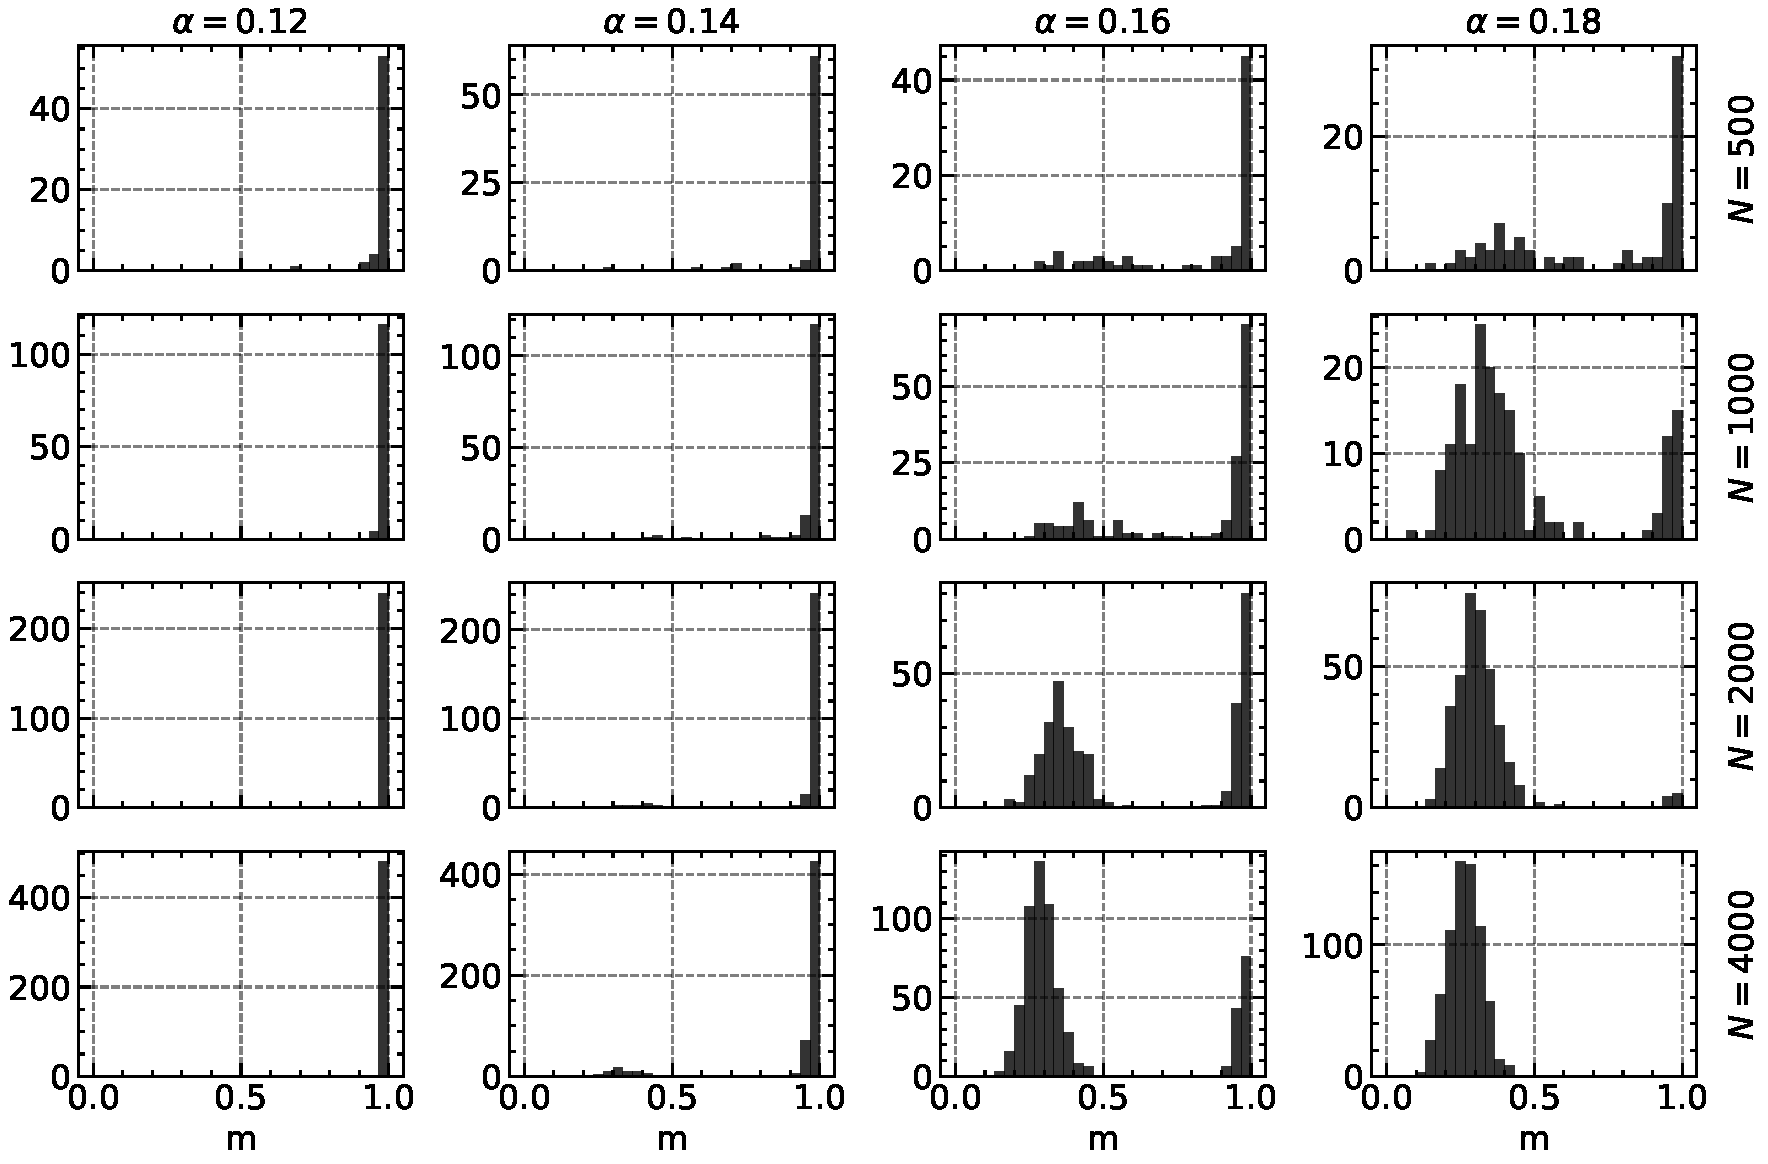
\includegraphics[width=\textwidth]{figures/overlap_histograms.pdf}
    \caption{resultados obtenidos para el overlap en función de \(N\) y \(\alpha\). Se observa que para \(\alpha = 0.12\) la red recupera los patrones correctamente para todo N. Sin embargo, a medida que se incrementa \(\alpha\), se obtienen valores de \(m < 1\), donde es más notorio para \(N = 2000\) y \(N = 4000\), lo que indica que la red no recupera correctamente todos los patrones originales.}
    \label{fig:ej1}
\end{figure*}

Además, se comparó el tiempo de convergencia de la dinámica secuencial con la dinámica paralela. Los resultados obtenidos se muestran en la Figura \ref{fig:ej1_time}.

\begin{figure} [htbp]
    \centering
    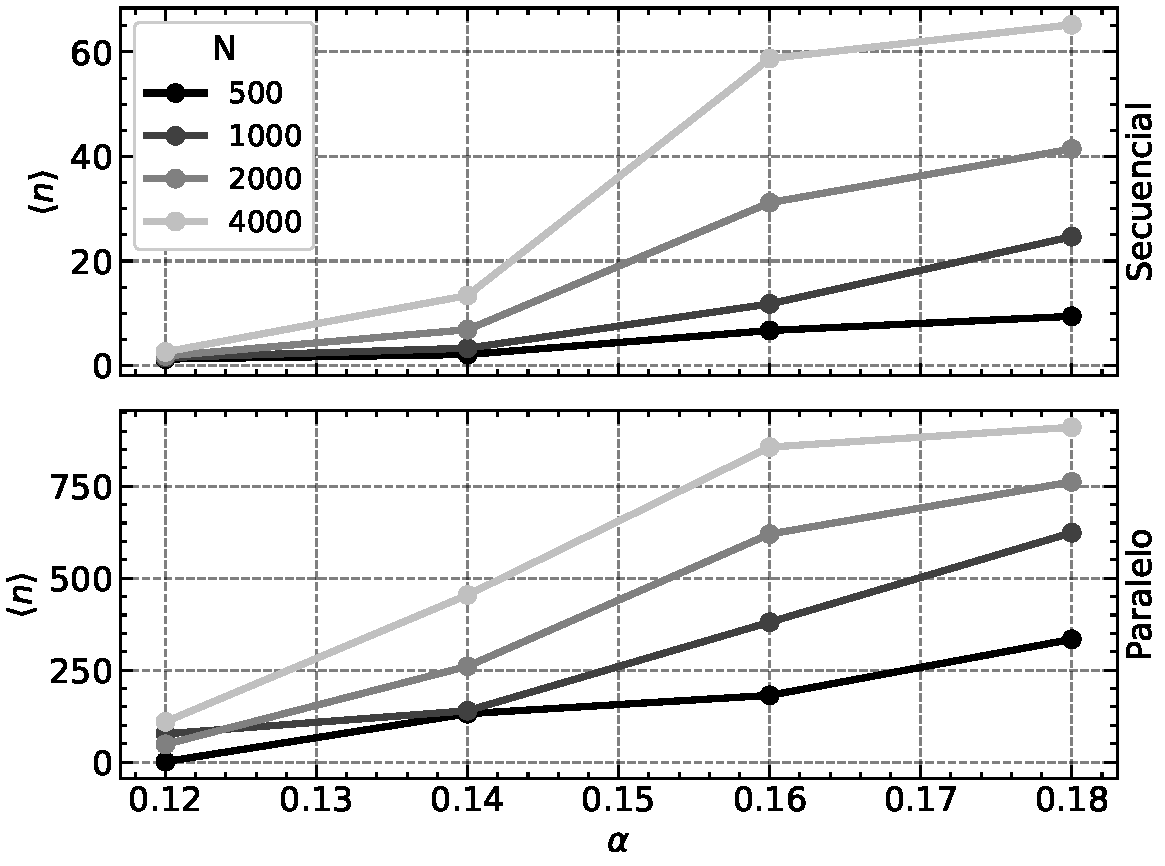
\includegraphics[width=0.5\textwidth]{figures/overlap_vs_alpha.pdf}
    \caption{comparación del número de iteraciones promedio de convergencia entre la dinámica secuencial y la dinámica paralela para cada N y \(\alpha\). Se observa que la dinámica secuencial converge más rápido que la dinámica paralela.}
    \label{fig:ej1_time}
\end{figure}

La evolución de la dinámica hacia el punto fijo se limitó en un número máximo de 1000 iteraciones por cuestiones de tiempo de cómputo. Es decir en caso de no converger en 1000 iteraciones, se consideró que la red no recuperó el patrón original. Por lo tanto, como se muestra en la Figura \ref{fig:ej1_time}, en la dinámica paralela para \(\alpha = 0.18\) y \(N = 4000\) se obtiene un número de iteraciones promedio \(\sim 950\), lo que indica que alguna de las iteraciones pudo no converger y estar limitada por el número máximo de iteraciones del algoritmo.



% --------------- EJERCICIO 2 ---------------------
\subsection*{Ejercicio 2}
En este ejercicio se estudió la dinámica de una red de Hopfield con ruido. Para ello, se generaron patrones \(x_i^\mu\) con \(i = 1, \ldots, N\) y \(\mu = 1, \ldots, P\), donde cada elemento de los patrones es \(\pm 1\) generados con igual probabilidad. En este modelo, la dinámica está gobernada por una componente aleatoria dada por

\begin{equation} \nonumber
    \text{Pr}(s_i(t+1) = \pm 1) = \frac{\exp(\pm \beta h_i(t))}{\exp(\beta h_i(t)) + \exp(-\beta h_i(t))},
\end{equation}

\noindent donde \(h_i(t) = \sum_{j=1}^{N} \omega_{ij} s_j(t)\) y \(\beta\) es un parámetro que controla la probabilidad de que el patrón \(s_i(t+1)\) sea \(\pm 1\). 

Se recorre la red aplicando esta regla un número de iteraciones fijo ya que la dinámica es estocástica. Luego de recorrer la red se calcula el \textit{overlap} m entre el resultado de la red y los patrones originales según la ecuación mencionada en el ejercicio anterior.

El procedimiento mencionado se consideró N = 4000 y p = 40, variando el parámetro \(T = 1/ \beta = 0.1, 0.2, \ldots 2\) en donde se evolucionó la dinámica durante 10 iteraciones. Los resultados obtenidos para el overlap promedio en función de T se muestran en la Figura \ref{fig:ej2}.

\begin{figure} [htbp]
    \centering
    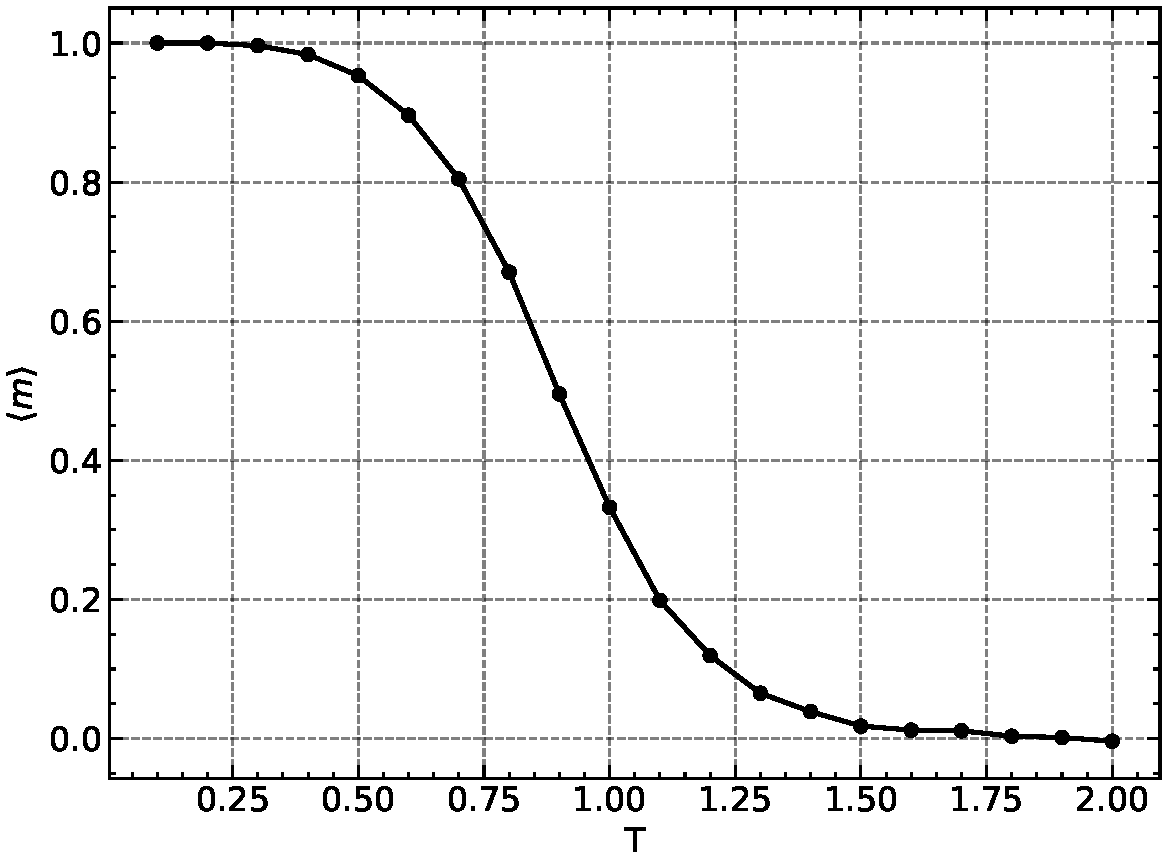
\includegraphics[width=0.5\textwidth]{figures/overlaps_ej_2.pdf}
    \caption{resultados obtenidos para el overlap promedio en función de \(T = 1/\beta\). Se observa que a medida que se incrementa \(T\), el overlap disminuye.}
    \label{fig:ej2}
\end{figure}

Para los valores de T más pequeños, el overlap tiende a 1 lo que indica que se puede recuperar los patrones. Sin embargo, a medida que se incrementa T, el overlap disminuye. Esto se debe a que a T altas, \(\text{Pr} (s_i(t+1) = \pm 1) \sim 0.5\), por lo tanto en promedio la mitad de las veces el overlap es \(\sim 1\) y la otra mitad \(\sim -1\), lo que resulta en un valor de overlap promedio \(\sim 0\). El hecho de que la transición sea suave y que no sea exactamente 0 se debe al tamaño finito de la red y a la cantidad finita de patrones utilizados.



\end{document}